\section{System Modeling}


\begin{figure}[H]
    \centering
    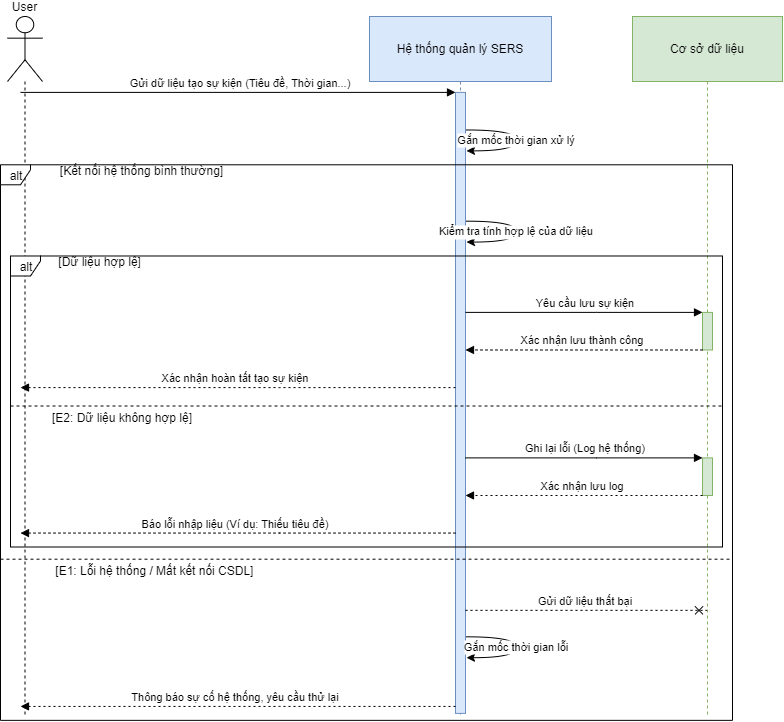
\includegraphics[width=0.7\textwidth]{pictures/seq1.png}
    \caption{Sequence Diagram mô tả cho việc tạo mới event}
\end{figure}

\begin{figure}[H]
    \centering
    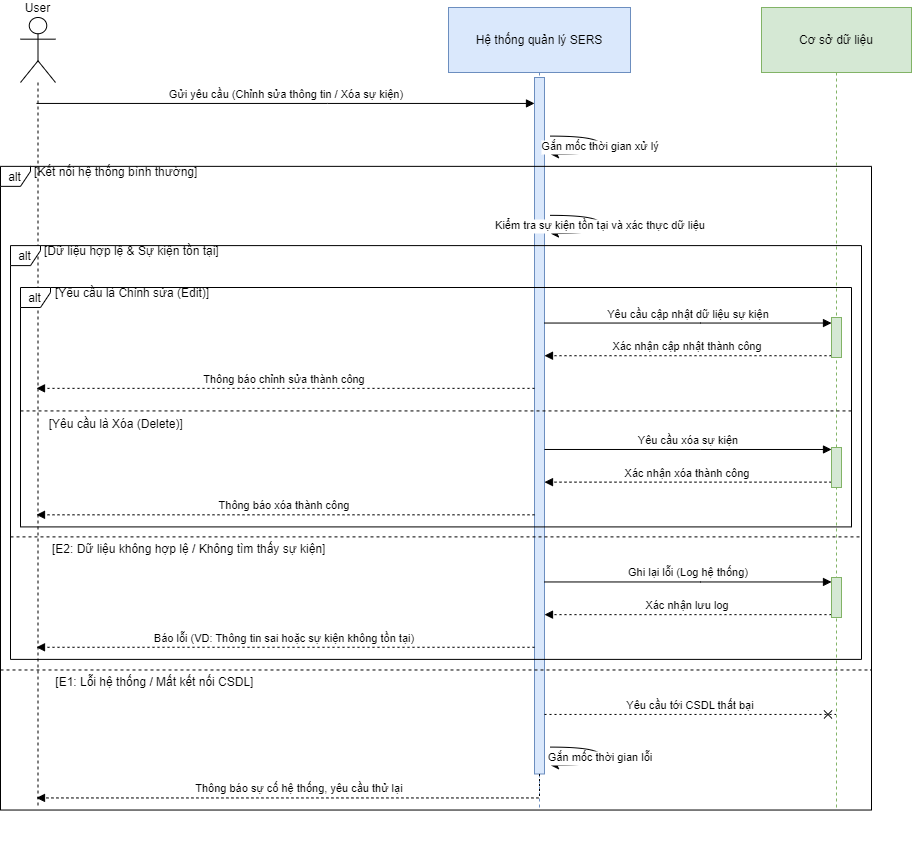
\includegraphics[width=0.7\textwidth]{pictures/seq2.png}
    \caption{Sequence Diagram mô tả cho việc chỉnh sửa và xóa event}
\end{figure}

\begin{figure}[H]
    \centering
    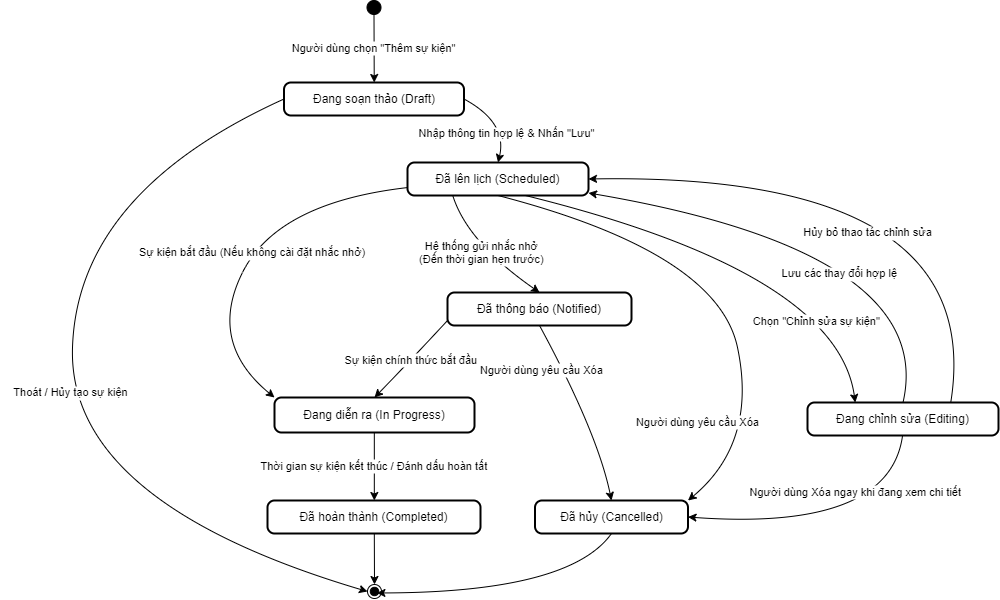
\includegraphics[width=1\textwidth]{pictures/statedia.png}
    \caption{State Diagram mô tả vòng đời các event}
\end{figure}

\begin{figure}[H]
    \centering
    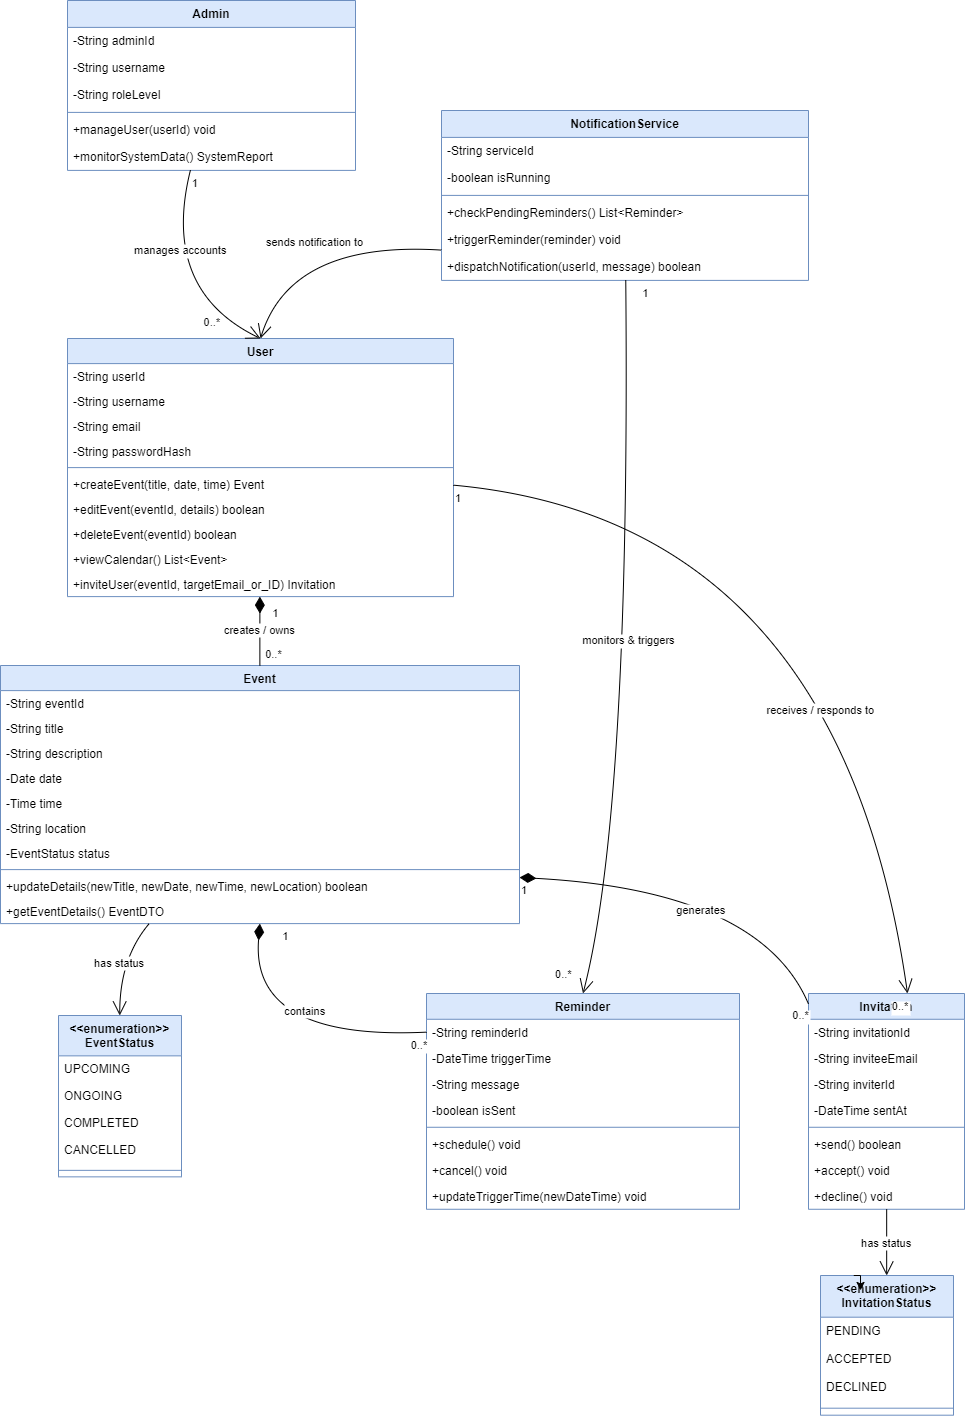
\includegraphics[width=0.85\textwidth]{pictures/classdia.png}
    \caption{Class Diagram mô tả cách hiện thực các trong hệ thống này}
\end{figure}